\documentclass[11pt,twoside,bibtotoc]{scrartcl}
%\documentclass[12pt, a4paper]{article}

\newif\ifpdf
\ifx\pdfoutput\undefined
\pdffalse % we are not running PDFLaTeX
\else
\pdfoutput=1 % we are running PDFLaTeX
\pdftrue
\fi

\ifpdf
\usepackage[pdftex]{graphicx}
\else
\usepackage{graphicx}
\fi

\usepackage{ucs}
\usepackage[utf8x]{inputenc}
%\usepackage[T1]{fontenc}
\usepackage[english]{babel}
%\usepackage{german}
%\usepackage{longtable}
%\usepackage{tocbibind}
%\usepackage{makeidx}
\usepackage[pdftex,pageanchor,colorlinks,pdfborder=0,breaklinks,urlcolor=blue]{hyperref}
\usepackage{amsmath}
\usepackage{amsfonts}
\usepackage{amssymb}
\usepackage{units}
%\usepackage{pdfsync}  % enable tex source and pdf output syncronicity
%\usepackage[all]{xy}
\usepackage{multicol}
%\usepackage{rotating}
%\usepackage{wrapfig}
%\usepackage{subfigure}
%\usepackage{listings}

\usepackage{geometry} % to change the page dimensions
\geometry{a4paper}
\geometry{textwidth=16.0cm,textheight=24.5cm}
\geometry{left=3.0cm,twoside}
\parskip=0 cm
\parindent=0.0cm

\renewcommand{\baselinestretch}{1.2}

\newcommand{\mytitle}{Tool support for user testing of stereoscopic fatigue}

\usepackage{fancyhdr} % This should be set AFTER setting up the page geometry
\pagestyle{fancy} % options: empty , plain , fancy
\fancyfoot{}
\fancyfoot[LE,RO]{\textrm{\thepage}}
\fancyfoot[LO,RE]{\textit{Roethlin, G. 2008}}

\renewcommand{\labelitemi}{-}

\newcommand{\todo}[1]{{\LARGE TODO: #1}}

% Depth of the TOC
%\setcounter{secnumdepth}{3}
%\setcounter{tocdepth}{2}

\hypersetup{
    pdftitle={\mytitle},
%    pdfsubject={Subject of the document}, % Subject 
    pdfauthor={Gerhard Roethlin},              % Author
    pdfkeywords={master, fatigue testing software, stereo vision},       % Keywords
}

\title{Master Thesis: \mytitle\\
{\large Designing and implementing a flexible and extensible testing framework}}
\author{\normalsize Gerhard R\"othlin 
{\texttt{\href{mailto:cbreak@the-color-black.net}{cbreak@the-color-black.net}}}}
\date{2008.01.07 - 2008.07.07}

\ifpdf
\DeclareGraphicsExtensions{.pdf, .jpg, .tif}
\else
\DeclareGraphicsExtensions{.eps, .jpg}
\fi

\begin{document}

\maketitle

\begin{center}
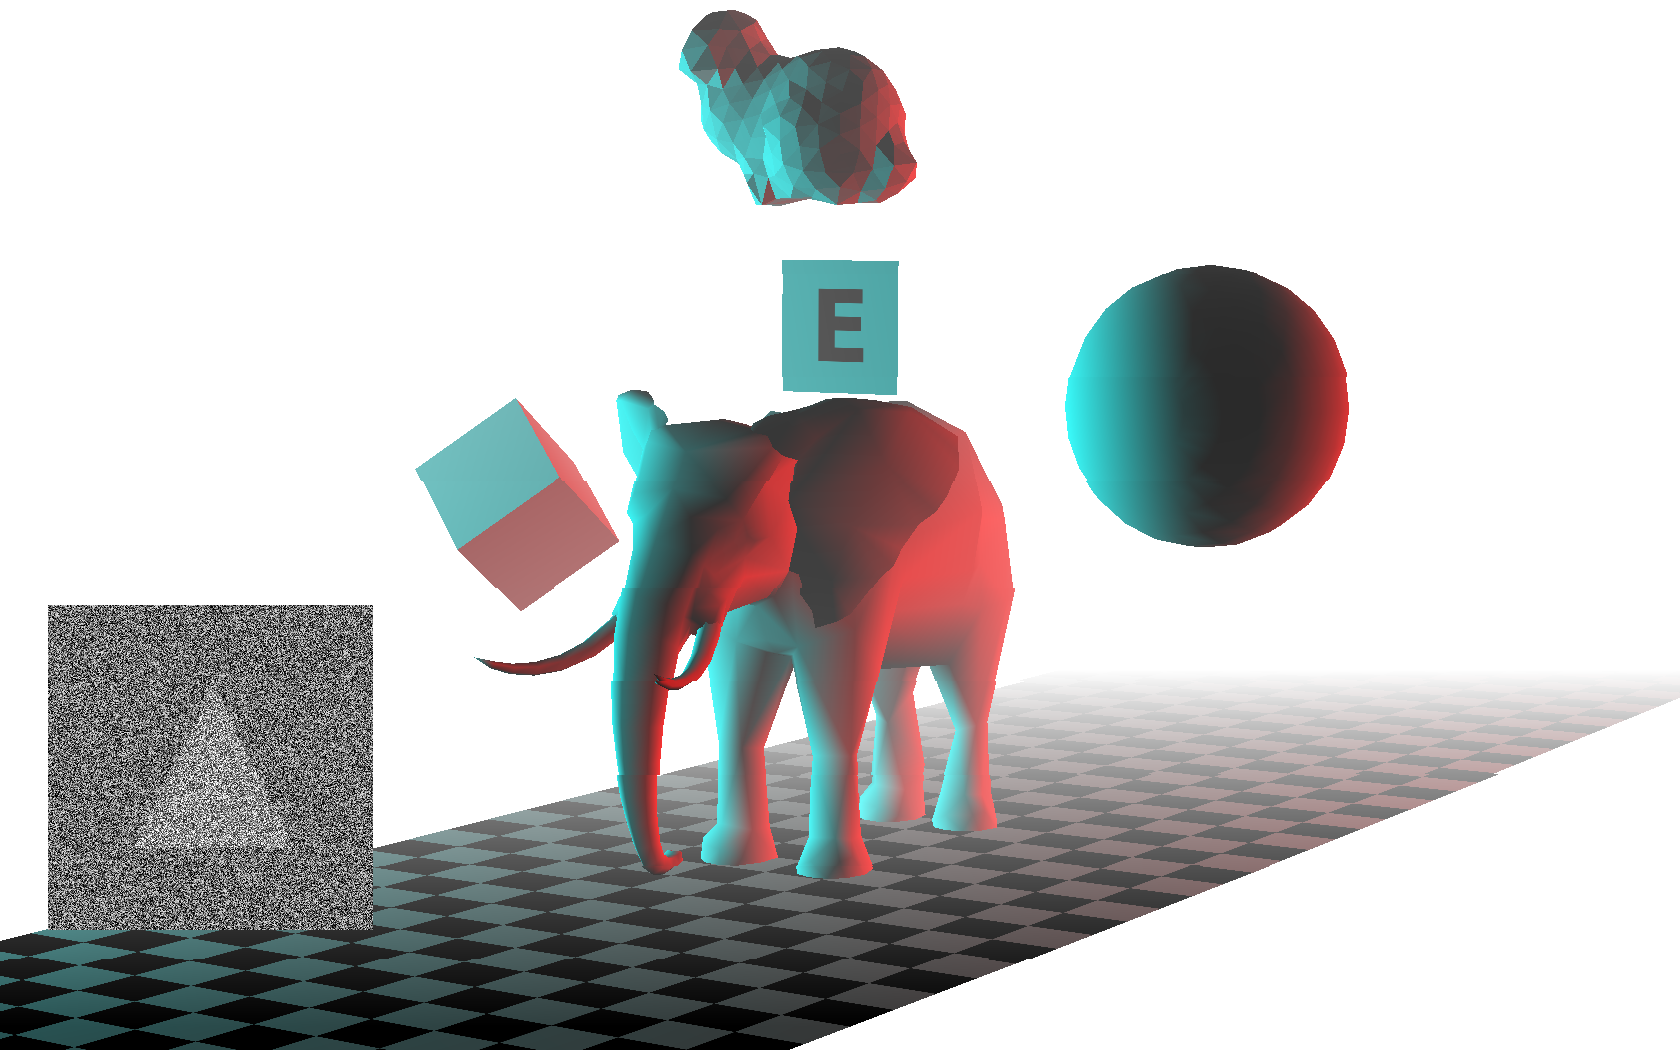
\includegraphics[width=15cm,clip,trim=0cm 0cm 0cm 0cm]{media/title.png}
\end{center}

\begin{multicols}{2}

\section{Abstract}
\paragraph{}
 \begin{abstract}
Viewing stereoscopic movies or images is unnatural. The focus and vergence of the eyes have to be decoupled. This strains the eyes, and can lead to fatigue, which makes the consumption of stereoscopic information over longer periods of times hard. But what are the physiological and psychological limits of stereoscopic viewing fatigue? And how can stereo images be composed to reduce fatigue?

Topic of this thesis is to write a Tool that enables exploration of those and similar other questions by providing a flexible and extensible framework for user testing. It is currently unclear how fatigue can be measured properly, and what scenes can be used to specifically test fatigue. Finding out which methods work and which do not is also part of this thesis.
\end{abstract}
\section{Introduction\label{Introduction}}
\paragraph{}
Researching the effect of the viewing of stereoscopic stimuli requires a different tool than usual user testing. The stimuli have to be more complex, and more dynamic. While traditional tests only require simple input and don't need to react on it, changing the stimuli based on what happened is often a requirement for the tests planed in stereoscopic vision research.

The following sections will introduce several examples of use cases, tests in which the framework should enhance the procedures and lessen the work done in test design and execution.
In the features section, some important abilities needed in those tests are detailed.

\subsection{Use Cases}
\paragraph{}
Before writing a program, one has to understand for what the program is to be used. The following examples illustrate the tests for which this framework has to be able to be used.

\begin{description}
\item[Focus]
The most basic test is to validate if a participant can focus and fuse on a target at an arbitrary location in a stereoscopic scene.
This is important in many other tests, where focus and binocular fusion has to be ensured.

\item[Fusion limit]
This test is used to ``test out'' the limits of fusion of a subject.
Knowing the limits, an experiment can be changed, or subjects can be classified or rejected.

\item[Fatigue and Continuous depth]
In this test two targets are shown resting on a ground plane, at three depth locations.
The targets show information that can only be decoded under fusion.
Measured is the reaction time of the test subject.
Before the test, after the test, and in the middle of the test a questionnaire is showed.
Difficulties include the complicated randomisation rule and the questionnaire.
For more details see section \ref{ExampleFatiguePilot}.

\item[Pinning]
Pinning is a border violation problem in stereoscopic images.
Testing it requires displaying various shapes and objects at locations near the border, in front or behind the parallax plane.
Texture can heavily influence how pinning is perceived.
Moving and rotating the objects can further help understanding the problem.

\item[Motion Sickness]
Testing the effect of motion in stereoscopic movies is important for understanding the creation of a pleasant or exciting viewing experience.
Simulating and testing requires the ability to interactively move both camera, and objects in a scene.
Motion should also be pre-definable, possibly as formula or as smooth movement along a curve.

\item[Testing Scenes]
When designing an experiment, being able to interactively change details of the scene, and get immediate feedback how it looks is invaluable
Scenes that are not used to test subjects, but to test the testing procedure do not require logging, instead they need interactivity and real time control.
\end{description}


\subsection{Features}
\paragraph{}
To implement the use cases in the previous sections, the framework has to contain high level functionality, some of which is listed here.

\begin{description}
\item[User interaction]
The test subject and what it does is the main interest of studies.
As such, the possibilities of interactions should not be arbitrarily constrained, but instead be as wide and flexible as possible.
The most basic interaction is by using the keyboard and the mouse.
In this group also fall devices that emulate them, such as joysticks track balls or touch sensitive screens.
More input vectors are imaginable, ranging from voice input over body movement to sensory data of the test subject.

\item[Logging]
Logging is the core of a test, it represents the data that the scientist is after.
As such, it has to be both exact and flexible.
A core requirement is that everything that happens, can be logged.
The log should be usable for any kind of test, and still be simple enough to understand and analyse.

\item[Survey]
While measurements of timing and correctness try to create an objective result, subjective feedback can not be neglected.
Popular in research are questionnaires, simple questions with answers on a given scale or in a given set of possible answers.

\item[Stereograms]
Stereograms encode depth information in a pair of 2D images.
So called auto-stereograms even manage to do this with one single image.
The depth information in a stereogram can only be extracted under binocular fusion, which makes it the perfect tool to ensure fusion.
Generating stereograms of various types and sizes is therefore a requirement in many tests.
See section \ref{Stereogram} for a detailed description of stereograms, and how they are implemented.

\item[Arbitrary object support]
Displaying a wide range of objects is required in many tests, simple planes, cubes and pictures are rarely enough.
But implementing all possible shapes is not possible, so loading already created shapes offers all the desired flexibility.
Texturing and introspection of imported objects are important features.

\item[Camera and Object motion]
The camera and all objects have to be movable, both instantaneous and smooth.
Movement should be definable in many ways, for example as function, as path, or as interactive code that reacts on user input.

\item[Depth Cues]
Viewing stereo is not only rely on binocular stereopsis, there is a wide range of cues that help seeing depth.
Those might be beneficial for a test, or influence the outcome in an undesired way.
Being able to enable and disable individual cues would be extremely useful.

\item[Randomisation]
Many parameters of a test have to be randomised, position of objects, color or shape of an image or the expected answer of a test.
But just randomising is not enough, often it is required to randomly permute a set of possibilities to create a balanced test.
In some cases even this is not enough, random orders have to be computed based on complex rules.

\item[Ease of use]
While not a singular feature, it is never the less very important that a product is easy to use.
If a product is too complicated to be used, it is useless, no matter how powerful it is.
The usability of a test is in the responsibility of the test designer, but making the creation of the test as simple and intuitive as possible is the job of the tool.
Increasing the usability ranges from creating a simple consistent user interface that offers basic functionality over adding powerful and extensible scripting capabilities for power user, to writing good documentation.
\end{description}

%\part{Design}
\section{Design\label{Design}}
\paragraph{}
Implementing a flexible and powerful framework for user testing of stereoscopic problems requires a design that accounts for some special requirements. To find out what those requirements are, several tests where designed and executed. The design of the application was adapted to be fit for use in those and many other imaginable tests.

\paragraph{Creation}
The framework is split into three parts: The test design part aids with the construction of the test scene. A scene is a description of stimuli, possible inputs, and reactions to them. Traditional tests in this area show a series of pictures, requiring user feedback for each, while measuring the response time and the correctness. Stimuli are often precomputed and only consist of a single pixel image.

The requirements for stereoscopic test are different: It is not feasible to manually prepare stimuli, especially if complexe interaction is required. A method to generate them on the fly is needed.
Section \ref{sceneRep} describes how the look of a scene could be represented.

\paragraph{Testing}
The testing part is the most important. It displays stimuli and logs the user replies, reacting in a way that is defined by the designer of the test. While traditional tests only follow the question-response pattern, stereoscopic user tests often require more: Trials often have to be randomized with several constraints, simply randomizing might lead to overlaps, or imbalances in dependent properties. All parameters of the stimulus have to be directly or indirectly controllable based on user input such as movement of stimuli, movement of the camera, or visibility of objects.

\paragraph{Analysis}
Analysing the gathered data is the third part. This is usually done in a combinataion of Microsoft\texttrademark\ Excel\texttrademark\ and highly specialized data analysation methods such as Anova. Both are sophisticated and well known by the users.

The easiest way to achieve compatibility with the known procedures is to produce data in a format, that is evaluatable in those tools. A log transformation program can take care of this in most tests: The time stamp based logs get parsed, and challenge-response times get measured and written in a format importable by spread sheet applications.

Some tests might not follow this pattern, and the data has to be analysed in a different way.


\subsection{Representation of a Scene\label{sceneRep}}
\paragraph{}
Scene graphs are used to store scenes in a structured way. They have been continually developed since their invention\cite{scenegraph} to account for spatial, state, hierarchy and other properties. Many scene graph libraries exist, but they are usually focused on a specific field, and part of a bigger framework.

To be able to control inconsistencies such as individual depth cues, it is required that the scene graph can represent these. Nodes could add or remove cues for their children, giving a maximum of control to the users. Scene graph libraries do not support those requirements. Designing a simple scene graph is required.

\subsubsection{Node types}
\paragraph{}
Scene graphs are tree structures consisting of nodes with zero or more child nodes. The scene itself is typically the root node, while actual rendered objects often are leaves. The following nodes are planed to be implemented in the framework.

\begin{description}
\item[Rectangle] A primitive geometry node, which has the shape of a parallelogram. The node can reference a texture, which gets mapped on it's surface.
\item[Parallelepiped] A primitive geometry node, which has the shape of a parallelepiped (parallelogram prism). As it's parent it can be textured.
\item[Pixelplane] A primitive geometry node. It is used to draw pixel exact images at any position in space. It requires a texture to be visible. Pixelplanes are point shaped, and therefore are not influenced by scaling and rotation.
\item[Text] A primitive geometry node. It draws text at any position in space, similar to Pixelplanes.
\item[Mesh] A primitive geometry node who's geometry is defined by a mesh. The mesh can contain vertex normals and vertex texture coordinates. A texture can be mapped on the object. It might be desirable to also include vertex color.
\item[AffineTransformation] A group  node. It contains other nodes, which it can affine transform by directly manipulating the matrix stack.
\item[Camera] A group node. It contains other nodes, which are rendered by this camera instead of the global camera. This is used to control projection cues in a consistent way. Has to reset the depth buffer.
\item[DepthBuffer] A group node. Disables or enables the use of the depth buffer for all contained elements. This is used to disable occlusion clues. Can reset the depth buffer.
\item[Lighting] A group node. Enables lighting and a light source with controllable parameters for all sub nodes. This is used to enable lighting depth cues.
\item[Atmosphere] A group node. Enables the fog equation and controls its parameters. This is used to enable aerial depth cues.
\end{description}

\paragraph{}
The following nodes are problematic and might be hard to use, implement and understand due to their side effects.

\begin{description}
\item[XSize] A group node that scales objects to add or remove depth cues caused by perspective projection. It can be implemented on object (scale object individually, without consider intra object depth) or space level (scale  as function of depth, which is similar to a camera projection). Either way has it's own problems.
\item[XOffsest] A group node that moves objects it contains as function of their camera distance. Can be used to add or remove height-of-field, convergence or motion parallax cues.
\end{description}

\subsubsection{Node organisation}
\paragraph{}
\todo{Write about simple trees, parallel scene graphs, object soup}


\subsection{Mechanics of a Scene\label{sceneMech}}
\paragraph{}
\todo{Write about what makes a scene move, the code/interaction. Write about Procedual(LUA) and Finite-state-machine(Custom)}


\section{Cues\label{Cues}}
\paragraph{}
Seeing stereo is not only based on binocular stereopsis.There are several aspects of the visual impression that allow the perception of depth. Common depth cues include accommodation, aerial perspective, binocular disparity, convergence, height in visual field, motion perspective, occlusion, relative size, and relative density. In addition others have been suggested, such as linear perspective, light and shading and texture gradients.%, kinetic depth, kinetic occlusion and disocclusion, and gravity.

Cutting and Vishton\cite{DepthCues} analyzed nine of these depth cues to asses their relative strength. Those cues will be described in the following paragraphs, and their reproduction or elimination on screen in a digitally generated scene is discussed. The use of OpenGL or a similar technology is assumed, techniques like ray-tracing or vector based painting may require different methods.


\subsection{Projection based cues}
\paragraph{}
These cues are caused by the way the 3D world gets projected onto the 2D surface of the retina.
Even though the reason that each of them exists is the same, the way they are evaluated and their reproduction is different.

Most projections\cite{proj} that are in use, map a ray in the world space onto a single point in the image space. Parallel Projection\cite{parallel} and Perspective Projection\cite{perspective} are the most commonly used methods. Physical optics use a projection similar to perspective projection.

Since all the following cues are generated by the same cause, enabling and disabling each is not possible in a consistent way. There are two basic ways to get individual control anyway: Use one projection method for all parts of the scene, but compensate to remove or add clues. Or use one projection method for every part of the scene, and compose the resulting image. Careless use of either method can cause conflicts such as pinning, rivalry, or the inability to fuse the image.


\subsubsection{Relative size}
\paragraph{Description}
The size of objects relative to each other is a strong clue for their distance, but it requires knowledge or assumptions about the size of an object. Due to the perspective projection, objects further away from a viewer take up less space in it's field-of-view. When seeing a human, it's distance can be estimated fairly accurately.

Seeing an unknown object requires comparisons with other objects in the scene. Upon seeing a number of cubes with different perceived sizes, and without prior knowledge of their size, one could assume similarity in size, and derive depth relations between them.

\paragraph{Reproduction}
Relative size only works when the perceived size of an object changes with it's distance. Using a perspective camera is an easy way to do this. When creating an artificial image, the size change can also be simulated by scaling objects based on their distance to the camera. In the case of OpenGL or most RayTracers, both parallel and perspective cameras are available.

\paragraph{Non-reproduction}
If the size of objects is not intended to change with their distance from the viewer, either choosing a parallel projection or compensating the projection based scaling by scaling the object size is needed.


\subsubsection{Relative density}
\paragraph{Description}
Relative density is closely related to relative size. It concerns the projected density of objects, which are distributed regularly. When such a group of objects change in depth, or take up different depth areas, their change in perceived density yield information about the depth change.

\paragraph{Reproduction}
If a perspective projection is used, relative density changes are calculated correctly. Introducing relative density clues into a scene that is rendered with a parallel projection requires non uniform scaling.

\paragraph{Non-reproduction}
Eliminating the relative depth cue from part of a scene that is parallel projected requires non uniform scaling of a group of objects. Both the position relative to each other, and the size relative to each other of the objects has to change.


\subsubsection{Height in visual field}
\paragraph{Description}


\paragraph{Reproduction}

\paragraph{Non-reproduction}


\subsubsection{Motion perspective}
\paragraph{Description}

\paragraph{Reproduction}

\paragraph{Non-reproduction}


\subsubsection{Convergence}
\paragraph{Description}

\paragraph{Reproduction}

\paragraph{Non-reproduction}


\subsubsection{Binocular disparity and stereopsis}
\paragraph{Description}

\paragraph{Reproduction}

\paragraph{Non-reproduction}



\subsection{Other cues}


\subsubsection{Occlusion}
\paragraph{Description}
Objects that are in front of other objects relative to the viewer are perceived to occlude the object behind. Even transparent or translucent objects often change the appearance of objects they occlude. This allows to infer depth ordering of objects. This clue is very strong, and it's range is the longest of all depth cues. It does however not allow to judge the distance between objects.

\paragraph{Reproduction}
Reproducing this depth clue digitally requires extra work, since most output media do not have a notion of depth. A traditional approach is the Painter's Algorithm\cite{painters}. Objects are ordered by depth and drawn from far to close. Ordering objects has performance implications, and is not always possible.
A newer method that does not require sorting is the Depth Buffer\cite{zbuffer} (also known as Z-Buffer). For every pixel it's associated depth value is stored. New objects only replace pixels further away.

\paragraph{Non-reproduction}
Not reproducing this clue is fairly straight forward. Disabling the depth buffer allows ordering objects according to preferred depth appearance, independently of their actual depth coordinates. Objects that are both behind and in front of an other object have to be segmented into pieces. This is most commonly the case when objects intersect.

Objects that consist of several surfaces might require internal ordering to appear correct, which is expensive. One way to resolve this problem is to clear the depth buffer after every object drawing. Depending on the size of the image this might be costly also.


\subsubsection{Aerial perspective}
\paragraph{Description}
Areal perspective is related with Occlusion: Objects far away from the viewer are often occluded by the atmosphere, be it air, smoke, fog or water. Consequentially, objects far away change their appeared color, losing saturation, and chroma.
Unlike most depth cues, it gets more effective as the distance from the observer increases.

\paragraph{Reproduction}
Reproducing this cue requires extra work. A common approach is to mix the object color with a fog color, depending on it's distance to the observer. This is cheap, and can be enabled per object\cite{fog}. Weights of the mixing is determined by a fog equation.

\paragraph{Non-reproduction}
Not reproducing this clue is easy, and it is not enabled by default. Explicit control over the appeared depth can be achieved by individually changing the fog equation for each object.


\subsubsection{Accomodation}
\paragraph{Description}
Accommodation is the change in the shape of the lens of the eye, to keep the perceived image of the world sharp\cite{accommodation}. It is coupled with convergence. Viewing stereoscopic material requires that the accommodation stays the same, since all image information comes from a screen at a fixed depth.

\paragraph{Reproduction}
Artificially generating the requirement that the human eye changes accommodation is hard. It requires optics in between the eye and the screen, or the changing of distance to screen depending on the object that is focused. Neither is practical.

\paragraph{Non-reproduction}
Not reproducing this cue is almost required. Everything seen on a screen requires the same accommodation to be viewed as the screen itself. If a constant accommodation requirement throughout the scene exists, a screen at a huge distance, or a convex screen can be used.

%\part{Implementation}
\section{Implementation\label{Implementation}}
\paragraph{}
This section presents selected implementation details, describes the technologies in detail, and the tradeoffs that where taken.

\subsection{Used Frameworks\label{frameworks}}
\paragraph{}
When developing an application, it is impossible to write everything from scratch.
Frameworks and libraries help developers not spending time on reinventing wheels,
but on finding solutions to the specific problems of their program.

\ER\ uses several libraries for window management, memory management, scripting and rendering.


\subsubsection{Qt\label{FrameworkQt}}
\paragraph{}
A big part of the functionality comes from the operating system and associated platform APIs.
This includes basic necessities like reading data from a file, drawing data to screen or specialized functionality like drawing a tree view, scaling images or managing tool windows.

\paragraph{}
All operating systems offer their own API to do some of those things.
\textit{POSIX} is supported on Linux, Mac OS X and Windows, but it only covers basic file IO, and nothing graphical.
Specific APIs like \textit{Mac OS X'}s \textit{Cocoa} or Windows' \textit{.Net} have a much richer feature set, but limit the application to that platform.
This might be acceptable for widely distributed end user applications where a fraction of potential users can be ignored,
but in a research environment the software has to be able to use existing hardware optimally.
A solution is \textit{Qt}\cite{qt}:

\begin{quotation}
Qt is a cross-platform application framework for desktop and embedded development. It includes an intuitive API and a rich C++ class library, integrated tools for GUI development and internationalization, and support for Java™ and C++ development.
\end{quotation}

\paragraph{}
An alternative would be to use \textit{Java} with it's associated APIs, but it's support for hardware accelerated drawing is lacking.


\subsubsection{Boost\label{FrameworkBoost}}
\paragraph{}
\textit{C++} is an old language, and has it's root in the language \textit{C}.
Neither has advanced memory management tools, be it a garbage collector like \textit{LUA} or \textit{Java}, or a reference counting system like used in \textit{Objective-C}.
Managing memory manually is a challenge, doing it wrong can cause crashes that are hard to debug.

A solution to this problem is offered by \textit{TR1}, an extension to the C++ standard library.
Boost\cite{boost} is a provider of a \textit{TR1} implementation.

\paragraph{}
\textit{TR1} contains among others a robust and flexible implementation of a set of shared-ownership smart pointers.
As long as a smart pointer to a memory location exists, it can be used like a normal pointer thanks to \textit{C++}'s operator overloading,
but as soon as all pointers to it go out of scope, the memory will be automatically deallocated.

\paragraph{}
An other useful feature in boost are function binders.
while standard \textit{C} functions and static functions can be pointed at by a simple pointer,
\textit{C++} class member functions require more data
(Method Pointers vary in size depending on compiler and platform, and can be 12 bytes or more).
Together with the strict type checking of \textit{C++}, this makes storing pointers to member functions complicated and inflexible.

With \textit{TR1}'s functional library, binding any kind of method or function and storing it is easily possible, while still retaining strict type checking.
This is used to implement callbacks.


\subsubsection{OpenGL\label{FrameworkOpenGL}}
\paragraph{}
Since the whole goal of the tool is to generate stereoscopic stimuli and present them to test subjects,
the graphical rendering framework is of tremendous importance.
In the beginning of graphical computers, programs drew everything on their own, and accessed the frame buffer directly.
In modern systems, drawing is highly abstracted and often hardware accelerated.

\ER\ requires the ability to draw 3D scenes and reproduce many effects such as lighting, cameras, atmospheric effects and other depth cues.
The goal is to be able to test both abstract scenes consisting only of few shapes and a limited amount of cues,
as well as scenes that contain many cues, and more closely approximate real visuals.
This is similar to what computer games use.

\paragraph{}
The only cross platform 3D drawing toolkit is \textit{OpenGL}\cite{opengl}, a standard developed by \textit{Silicon Graphics} in 1992.
It's a state-driven procedural C API that was extended with many additions to the standard since it's inception.
Many features of \textit{OpenGL} are accelerated by modern graphic cards, and allow real time animation rendering.

The \ER\ renderer uses \textit{OpenGL} for the scene output.
Objects paint them-selfs with OpenGL commands.
The offerings of the framework are not perfect, but it allowed to realize almost all desired features.
A more advanced anaglyph renderer would likely be possible to do with frame buffer objects and pixel shader, but that would exclude a wide range of older installations and hardware.


\subsubsection{LUA\label{FrameworkLua}}
\paragraph{}
It was clear from the beginning of the project that the only way to get the required flexibility to do anything, and test anything can not be achieved by simply defining a scene format and some animation paths.
Tests like a flight simulator for motion sickness require interactivity in complex ways.
The chosen solution was to use a programming language to specify interaction and mechanics of a test.
The design of a language is complex, and many scripting languages are already established, so it was decided to reuse an existing language.

Most scripting languages are either intended to be used in stand-alone scripts such as \textit{Perl} or various shell scripting languages.
\textit{Python} can be used as  embedded language, and offers a very rich API on it's own.
The downside is that it is huge and comes with many features that are not needed, which complicate
the integration into custom applications.

\paragraph{}
The chosen language is \textit{LUA}\cite{lua}, a small library designed to be used as embedded language.
It provides all basic features, comes with garbage collection, flexible syntax and powerful binding API.
It's syntax is easy to understand, but still offers enough sugar to use not only procedural, but also modular, object oriented or functional programming.
It's license is very liberal, which made it popular even in the comercial game industry.
The official project description emphasizes those points.

\begin{quotation}
Lua is an extension programming language designed to support general procedural programming with data description facilities. It also offers good support for object-oriented programming, functional programming, and data-driven programming. Lua is intended to be used as a powerful, light-weight scripting language for any program that needs one. Lua is implemented as a library, written in clean C (that is, in the common subset of ANSI C and C++).
\end{quotation}

\paragraph{LuaBridge}
While the \textit{LUA} C API is very powerful, it is also very low level.
Writing code that interacts with \textit{LUA} and especially code that is called by it requires following the calling convention of \textit{LUA}.
Manually handling the low level API helped with understanding the language better and finding problems,
but it also required to maintain two interfaces, one that exposes functions to \textit{C++} and a second set for \textit{LUA}.

\textit{LuaBridge} automatically generates this binding code in a very elegant way.
Unlike tools like \textit{tolua++} it does not require a preprocessor,
it uses template meta programming to generate wrapper code.
\textit{LuaBind} works similar, but \textit{LuaBridge} is smaller, easier to understand and has less dependencies.




\subsection{Program}
\paragraph{}
The class \lstinline{Program} encapsulates a test scene.
It contains the scene graph (see \ref{SceneGraph}) and the scene mechanics (see \ref{Mechanic}).

The program mediates user input and relays it to the engine
and handles loading and storing of a scene.

The scene also manages names.
Names are important especially for serialisation, since lua variables are referred to by name.
Uniqueness and validity is ensured, and reserved lua keywords are protected.

\paragraph{Internal interaction}
In the current implementation, the scene mechanic code accesses the scene graph directly,
and has references to the actual objects.
This makes modularisation more difficult, and makes it impossible to replace a whole scene graph with a duplicate.
An improvement would be to only refer to objects by name or with some sort of \textit{URI}.
Implementing such a scheme would require a huge effort especially due to the nature of the binding to \textit{lua}.
\textit{LuaBridge} does not support polymorphism.




\subsection{Scene Graph\label{SceneGraph}}

%\begin{figure*}[htb]
\begin{center}
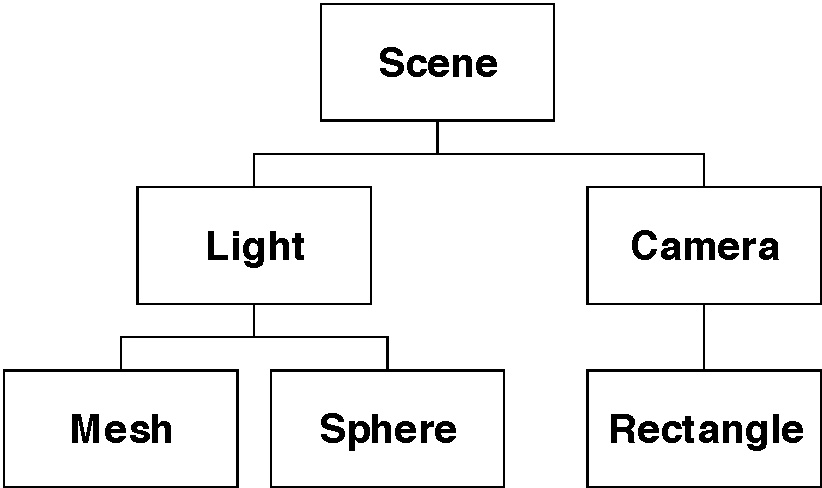
\includegraphics[width=7cm]{media/scene.pdf}
%\caption{A diagram of a possible scene graph.\label{imgScene}}
\end{center}
%\end{figure*}

\paragraph{}
The scene graph is organized by state.
State modifying containers contain visual objects.
The scene is a special container.

\subsubsection{Objects\label{ImplObject}}
Most objects represent a visual shape.
They are organized in an inheritance hierarchy, all based on the class \texttt{Object}.
This hierarchy heavily relies on polymorphism, so there are several virtual member functions that can be customized.

An object offers visibility through drawing itself in \textit{OpenGL} and persistence by writing itself to a stream as lua code.
An objects can also return a smart pointer to itself.
The method \lstinline{clone()} creates an exact deep copy of the object.
For the UI, it can return a dialog that directly changes the parameters of the object.
Other classes can install handlers into an object to be notified when it is modified.

\paragraph{Mesh}
The mesh node is the most flexible shape node.
It stores a mesh in a simple data structure, and draws this mesh as it's visual representation.
The mesh can contain texture and normal values in addition to vertex coordinates.

As input format, Alias Wavefront's Object format is used.
It is parsed by the obj library bundled with \ER.

To accelerate drawing, an \textit{OpenGL} display list is built.
To help drawing of different types of triangles, a small internal wrapper class is used.

\paragraph{Text}
The text node is a shape node that draws text.
It uses Qt's \lstinline{QGLWidget::renderText()} method to draw strings on screen.
This call uses the stencil buffer, so it is incompatible with the line-interlacing renderer that also uses the stencil buffer.

Alternative solutions to render text could include using pre-rendered bitmap letters as textures, or similar approaches.
It should be noted that good text rendering is complicated, modern fonts contain more than just simple letters and spacing data.

\paragraph{}
For more details please refer to the header file (see page \pageref{object.h}) or the doxygen documentation.
For an overview of objects, see section \ref{nodeTypes}.

\subsubsection{Containers\label{ImplContainer}}
\paragraph{}
Container nodes are a special subclass hierarchy of objects.
They can contain any kind of objects, including other containers, and modify how those objects are drawn.
Most nodes modify the \textit{OpenGL} stack, draw their contents and restore the previous stack.

\paragraph{Transformation}
The most used container class is likely \lstinline{AffineTransformation}.
It encapsulates a 4x4 transformation matrix and convenience accessors to easily modify the transformation.
Since normal shape nodes don't have a rotation property, transformation nodes are used to rotate them.

When a transformation node is drawn, it applies it's translation, multiplies it's matrix with the transformation matrix on top of the stack and draws it's contents.
The original top of the matrix stack is restored after the containing nodes have been drawn.

\paragraph{Light}
For lighting, the class \lstinline{LightNode} is used.
It applies a colored light with ambient light to all contained items.
This only makes sense if those items have normal vectors set.

For lighting, \textit{OpenGL}'s light model is used.
Not all parameters are exposed, but modifying or extending the class is possible.
Possible extensions could include spot light support or parallell light support.

The light node enables auto normalisation of vertex normals to compensate for possible scaling or other transformations of objects.
To define the object color easily, the \lstinline{GL_COLOR_MATERIAL} facility is used.
Colored objects automatically use this color as material color.
Due to a limitation in \textit{OpenGL}, only eight lights can be active at a time.
The depth of light nodes contained within other light nodes should therefore not exceed eight.

\paragraph{Fog}
To create atmospheric effects such as smog or fog, the class \lstinline{Atmosphere} is used.
It is a simple wrapper to \textit{OpenGL}'s \lstinline{GL_FOG} facility.
The same three types of foc are supported, and all parameters used by the foc facility can be set.

\paragraph{Camera}
The class \lstinline{CameraNode} is a powerful tool in creating non-consistent scenes.
It projects contained sub-objects with it's own camera instead of the scene camera.

It is implemented by loading the internal camera into the projection matrix stack, drawing the contained objects with this camera, and then restoring the original projection.

Due to the limitations of \textit{OpenGL}, the number of recursions is limited by the maximal depth of the projection matrix stack.
Since there is no benefit in recursing camera nodes, users should not do it to prevent problems.

For more information on cameras, see \ref{RendCamera}.

\paragraph{Depth Buffer}
The class \lstinline{DepthBuffer} is the only container subclass that does more than modifying and restoring \textit{OpenGL}'s state.
It clears the depth buffer after every sub object is drawn.
The depth ordering of objects on screen is therefore in draw order.
Object internally, the depth order is still maintained by the depth buffer, so the front- and back-face of objects is maintained.


\subsubsection{Surfaces}
Surfaces are used to place textures on objects.
The simplest surface is \lstinline{Texture}, a simple bitmap texture.
More sophisticated is the family of \lstinline{AbstractStereogram}, bitmap textures that are different depending on the side of the camera they are seen with.

The most prominent subclass is \lstinline{RandomdotStereogram}, a random dot texture generated from a depth map (see \ref{Stereogram}).
Other classes offer custom textures in depth-based stereograms, or custom stereograms.




\subsection{Mechanic\label{Mechanic}}

%\begin{figure*}[htb]
\begin{center}
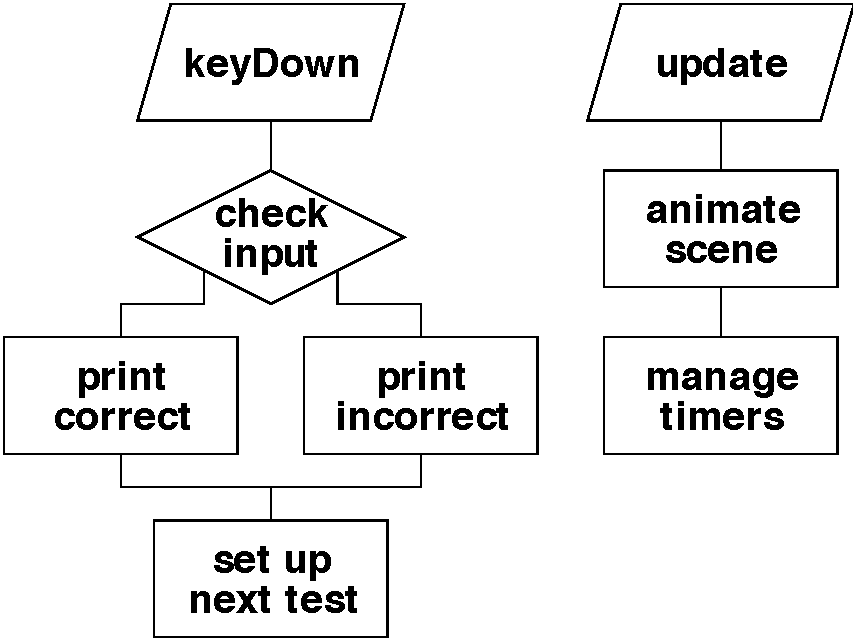
\includegraphics[width=7cm]{media/code.pdf}
%\caption{A diagram of a possible scene graph.\label{imgCode}}
\end{center}
%\end{figure*}

\paragraph{}
In the current version, scene mechanic is closely tied to Lua.
The interaction of the scene with the subject as well as internal actions such as animation are defined in \textit{lua} script, and executed by the \textit{lua} engine.

By modifying the class \lstinline{Program} it would be possible to replace lua with a custom interpreter for another language.
A graphical programming launguage or a key-frame interpolation class are possible replacements.

\subsubsection{Event Model}
\paragraph{}
Lua does not have a run loop or a main function.
It consists of code that is executed on load and functions that are called from \ER.
Once a scene has done the desired actions it is expected to return control to the program.

To easily integrate into \ER's model, event handler functions can be registered to receive notifications and execution control.
Three event handlers are commonly used: \lstinline{keyDown}, \lstinline{keyUp} and \lstinline{update}.
\lstinline{keyDown} is called when ever a key is pressed.
\lstinline{keyUp} is called when the key is released again.
The \lstinline{update} event is called in regular intervals, currently roughly thirty times per second.

\subsubsection{Binding}
The class \lstinline{LuaProxy} encapsulates the \textit{lua} engine.
It contains glue code to bind functionality from \textit{lua} to \textit{C++} and manages the event handlers.
Objects (see \ref{ImplObject}) are bound to lua with the \textit{LuaBridge} library.
This library handles almost all of the bridging, only in special cases, like enum parameters, objects have to provide custom methods.




\subsection{Rendering}
\paragraph{}
Rendering the scene into a perceivable image is one of the core jobs of the application.
Realizing effects that approximate both real movie footage and the wishes of the user is often hard, or even impossible.
The implementation is closely tied to the abilities requested from the tool, many effects such as lighting or arbitrary depth ordering requires low level trickery with the chosen framework.

In addition, the scene does not only have to be rendered once but often twice.
Binocular vision infers depth relationships from slight differences in images taken from two separate viewpoints.

Section \ref{FrameworkOpenGL} discusses the choice of rendering framework.
Section \ref{RendCamera} discusses how a 3D scene gets mapped into a 2D image.
Section \ref{RendStereo} discusses stereo rendering methods.
Section \ref{ImplContainer} discusses the implementation of other effects.
For a high level description of many features see section \ref{sceneRep} on scene representation and \ref{Cues} on the topic of depth cues.


\subsubsection{Camera\label{RendCamera}}

\begin{figure*}[hbt]
\begin{center}
\subfigure[Perspective Cameras]{\label{CamPer}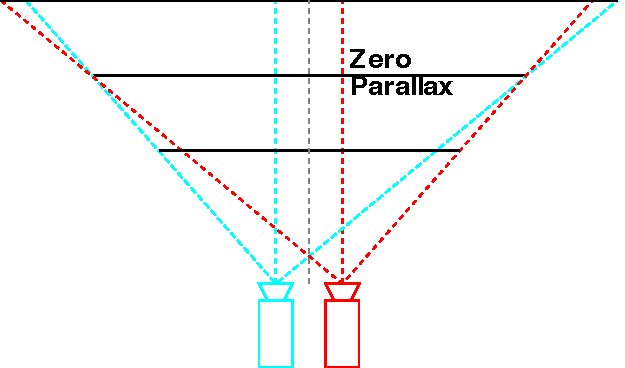
\includegraphics[scale=0.75]{media/camera-perspective.pdf}}
\subfigure[Parallel Cameras]{\label{CamPar}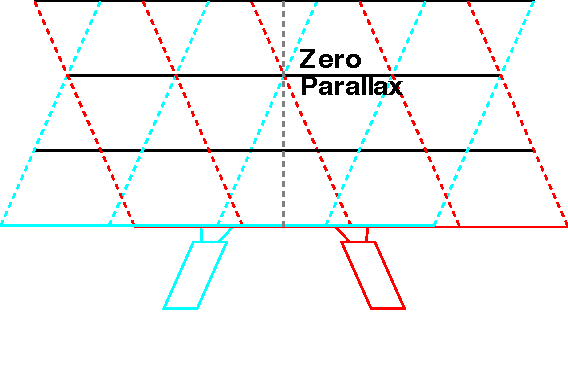
\includegraphics[scale=0.75]{media/camera-parallel.pdf}}
\caption{A diagram of the two main camera types}
\end{center}
\end{figure*}

\paragraph{}
To transform a 3D scene into a 2D picture on screen it is projected with a linear transformation.
The solution \textit{OpenGL} has is described below.
Real cameras often have non-linearities which can not be simulated with such a simplification.

To reproduce stereoscopically viewable content, two cameras are used, representing the left and right eye.
There are several ways to place the camera and parametrize the camera, two of which are implemented in \ER\ and described below.

\paragraph{OpenGL}
In \textit{OpenGL}, the projection matrix, a 4x4 matrix, defines the projection transformation.
This is the \textit{OpenGL} equivalent of a camera.
The projection matrix depends exclusively on the type of the camera.
The position and the direction of the camera is part of the modelview matrix.

Those matrixes are calculated by \textit{OpenGL}'s convenience function \lstinline{glOrtho()} or by calling \lstinline{glFrustum()} to directly set the matrix parameters depending on the camera type.


\paragraph{Perspective Cameras}
When working with physical cameras to create stereoscopic content, the main choice is whether to place the cameras parallel or converge them.

Converging helps with establishing the zero parallax plane, but causes problems with the separation of objects behind and in front of it.
Already at close range, the resulting images are strongly diverging, making the image unviewable.

Parallel cameras limit the divergence to the camera separation at the center of the image.
\ER\ uses parallel cameras.
With hardware parallel cameras, the zero parallax plane is set by shifting and cropping the two resulting images.
This is not needed in digital imaging, instead the projection matrix is adjusted to an asymetric frustum.
Figure \ref{CamPer} shows a schematic of this setup.

\paragraph{Parallel Cameras}
Parallel projecting cameras are not used in hardware.
They have some interesting properties that make them desirable in testing stereoscopic effects,
namely their elimination of relative size, motion and other perspective clues.

To get stereoscopic images that can be fused, converged cameras have to be used.
In \ER\ the camera projection matrix is skewed so that the projection planes of left and right camera are parallel, and the projection direction is non-perpendicular to it.
Figure \ref{CamPar} shows this setup.


\subsubsection{Stereo\label{RendStereo}}
\paragraph{}
Ideally, the output of the program is either intended to be viewed without binocular vision, or a projector solution is used.
Then the scene is simply rendered twice into different windows or in split screen.
If the used graphic hardware supports it, \textit{OpenGL}'s QuadBuffering can be used to easily drive many types of stereoscopic viewing systems.

\paragraph{Anaglyph}
For a quick and easy preview on any screen, anaglyph is the simplest method.
Many different variations of anaglyph are used, the most popular of which are red-blue and red-green coding.
A simple implementation could draw only the red channel of the image intended for the left eye, and the green and blue channel of the right eye.
Unfortunately this leads to rivalry when rendering scenes that contain objects that consist mostly of those colors.
This method is the one implemented in \ER\ by using \lstinline{glColorMask()} to lock writing to certain color buffers when drawing the left and right camera views.

A better way is to mix all colors of one side into its channel.
The loss of color contrast is made up with the better fuseability and the reduction in rivalry.
Other anaglyph methods such as Mayan\cite{Mayan} have a more sophisticated mixing algorithm.
Implementing them in \textit{OpenGL} requires storing image data of one side in a buffer and merge it with the other.
Reading data from the rendering buffer is slow, since auxiliary buffers are often not in the GPU memory.
It might be possible to implement anaglyph with fragment shaders, pbuffers or the color matrix pixel transfer operation.

\paragraph{Two-Side}
To drive projectors or similar systems that require two full frames, the two-side rendering method can be used.
The first implementation used two one-side render windows, but synchronizing update time was not feasible.
The time lag created artefacts with animation.

The new implementation changes the viewport of the rendering and draws both cameras side-by-side.
On a Two-Screen setup in full-screen, the window gets spread on both sides, giving each cameras one screen.
During most tests, this setup is used to drive two projectors with polarisation filters.

\paragraph{Line Interlace}
The 3D screen \textit{Trimon ZM-M220W} from \textit{Zalman} is a LCD screen that can display stereoscopic images with polarisation encoding.
The lines on the display are polarized with alternating directions.
With suitable polarizing glasses and proper head positioning, stereo images can be seen.

The encoding of the output image is a simple interlacing of alternating viewpoints.
The technique used to combine the left and right view uses the stencil buffer.
This is very fast, and requires no additional copying or other slow buffer operations.
Its drawback is the incompatibility with \textit{Qt}'s text rendering, that also uses the stencil buffer.

\paragraph{QuadBuffer}
\textit{OpenGL} itself supports a 3D technology called quad-buffering.
It offers not only a front- and a back-buffer as in traditional double-buffering,
but front- and back-buffers for both left and right eyed view.

Hardware support for this technology is expensive due to driver limitations implemented by the hardware vendors.
To use this output mode, a supported graphics card and driver is required.
The Quad-Buffer output mode was not tested with proper hardware and enabling quad-buffering on not supported hardware caused massive side effects with buffering.
This output mode should nevertheless work with a slight change in MainWindow's \textit{QGLFormat} creation.




\subsection{Stereogram\label{Stereogram}}
\paragraph{}
A stereogram is an image that contains separate data for the left and right eye. Specially crafted images can cause a binocular depth perception. The framework supports stereograms in various formats. The simplest case consists of two images, one for each eye. Several types of random dot stereograms are also available.

\subsubsection{Random dot stereogram\label{RDS}}
\paragraph{}
Random dot stereograms are a topic that has interested scientists since over a century\cite{AntRDS}. In the early 1960s they were introduced as stimuli into the modern neuroscience by Julesz\cite{BellRDS}. Unlike a normal stereogram, a RDS contains no monocular clues of the depth, or any clue about the stereoscopic image at all. This makes them the perfect tool to study binocular vision.

The two images of an RDS consist of a random pattern, usually dots. Since either image on its own is purely random, no information can be derived of it. When seen with binocular vision, depth can be seen. There are several different methods to create a random dot stereograms, but their principle is the same:
Based on depth information, parts of the pattern in one or both eyes are shifted on the horizontal axis.

\paragraph{Simple algorithm}
The first and most simple algorithm implemented is based on the original technique used by Julesz\cite{BellRDS}. A random pattern for the left eye is created, and also serves as the background in the image for the right eye. A subset of this pattern, which is defined by a mask, is shifted by a fixed amount of pixel. This is enough to create a pair of images that are on their own almost completely random, but produce a perceivable depth effect.

This approach does have problems: Areas whose contents are shifted have to be filled up again.
The chosen solution was to not move but copy the contents, so that there are duplicate patterns in the image.
Creating concave surfaces requires shifting the area in the image for the other eye, or there will be border conflicts similar to pinning.

Its advantage is that it's fast and easy to both implement and execute.
Memory access to the image buffers can be limited to one write per pixel, the pixel data for the shift can be cached in short ring buffer.

\paragraph{Advanced algorithm}
\begin{figure*}[htb]
\begin{center}
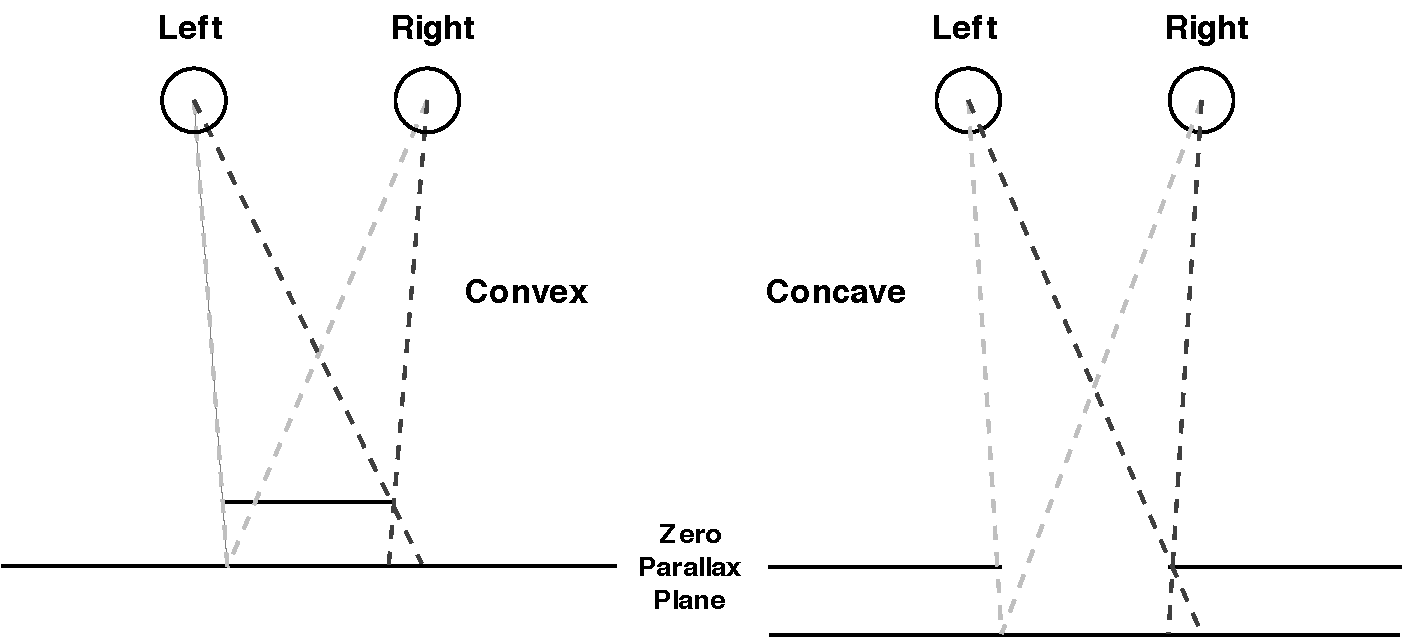
\includegraphics[width=15.5cm]{media/rds.pdf}
\caption{RDS of Convex and Concave surfaces can be created in different ways\label{ccRDS}}
\end{center}
\end{figure*}

\paragraph{}
The second algorithm is split into two parts, which deal with convex and concave stereograms separately.
This deals with subtle problems with partial occlusion (see figure \ref{ccRDS}).
It also uses different patterns for fore- and background.
Using pre-calculated patterns was loosely inspired by a paper from Gonzalez and Krause\cite{GenRDS}, which allowed different densities for object and background.

Using different colors for the foreground and the background makes the object defined in the depth map stand out. This helps visibility, but that way the shape of the object itself can not be used to validate fusion. Depending on the offset of fore- and background and the size of the random dot stereogram, it is not easily monocularly visible if the shape is convex or concave.

Both methods are simplified, the virtual cameras are always at the same relative position of the pixel in the depth map that is processed, similar to a parallel projection.

\paragraph{Convex}
The algorithm for convex shapes treats the depth map as a source to calculate the new position of pixel in a source pattern.
The calculated offset is used to displace the surface into the destination image.
The shape is shifted horizontally and appears to come out of the surface.
This is equivalent to tracking the surface of the object, and projecting the observed value onto the background (figure \ref{ccRDS}, left).
The same effect can be achieved by tracking the background, but in border cases one eye would see the background, while the other eye sees the foreground.

\paragraph{Concave}
The algorithm for concave shapes works slightly different.
It treats the depth map as a source to calculate the position of the pixel in a source pattern to place in the destination pattern.
The shape is not shifted, but its texture is.
It appears to go into the surface.
This is equivalent to tracking the background plane, and projecting the corresponding object pattern values onto the background (figure \ref{ccRDS}, right).
It can be achieved by tracking the object, but in border cases,  a point might come from the foreground for one eye, and the background for the other.

\subsubsection{Pattern stereogram}
\paragraph{}
Pattern stereograms are created similarly to random dot stereograms.
Instead of a random data source, they use a pre-computed pattern as foreground and background image.
This makes the shape stand out more and allows a high customizability of the pattern.
Possible sources include randomly generated noise images, photographed textures and randomly distributed shapes.




\section{Meshes}
\paragraph{}
An important requirement for the tool is, that it has to be able to display a wide range of stimuli. Not only the depth cues (see section \ref{Cues}) have to be individually controllable, also the possible shapes of objects have to span a wide range.

The tool supports only few basic object types, such as Pixel Planes (raster image data), parallelograms, and parallelepipeds. Implementing every desired type in code is neither feasible nor desirable.
Instead, the same approach as with textures is taken: An external tool that is familiar to the user is used to create a shape, and this shape is then loaded and displayed by the tool. By far the most commonly used method to store models is \textit{Mesh}. A mesh is a surface defined by points, which are connected by edges, to form faces. Other methods include \textit{NURBS}, \textit{Constructive Solid Geometry} and many types of \textit{Parametric Surfaces}. They are less popular, and often harder to handle than meshes.

There are a number of possibilities to implement this design. A mesh library can be used to load, render and modify meshes in an easy way. A scene graph library provides not only mesh support, but also the handling of whole scene hierarchies. Mesh importer libraries make it easier to parse models into a custom data format.


\subsection{Mesh Libraries}
\paragraph{}
Mesh libraries provide an API for loading, manipulating and rendering meshes. \textit{OpenMesh} is a very powerful library with a half-edge data structure. It offers a wide array of possibilities to customize storage, access and manipulation. It does not handle rendering.

\paragraph{}


\subsection{Mesh Formats}
\paragraph{}

\subsection{Mesh Creation}
\paragraph{}



\subsection{User Interface\label{ImplementationUI}}
\paragraph{}
The User Interface is implemented with \textit{Qt}'s extensive widget classes.
\textit{Qt GUI} aims to provide native looking controls on all platform.
An experienced user can tell the difference between native applications and one written with \textit{Qt}, but having only one interface for three platforms makes this drawback worth having.


\subsubsection{Main Window}
\paragraph{}
The main window contains the \textit{OpenGL} scene view, the menu bar (on Mac OS X the menu bar is at the top of the screen) and a number of detachable widgets.
The scene view shows the look of the currently executing scene.
The widgets allow changing the scene or give more information.

\subsubsection{Design}
\paragraph{}
The design widget shows the scene graph as tree view.
A tree view is a standard widget, a list with items that can be expanded into sub-objects.
It is bound to the scene graph by a helper class that translates the calls from the widget to the backend scene graph.

The tree view item model uses placeholder items for each item.
Those place-holder items contain pointers to the represented object, it is one of the few places where raw pointers are used.
As a consequence it is also the place where most of the crashes during development happened.
For a detailed description of the api read the documentation on \lstinline{QAbstractItemModel} and \lstinline{QTreeView}.

To keep the tree-view in sync with the scene graph, the notification system of objects is used.
Every object notifies it's containing scene before and after external parameters change.
Container objects have special events for changes of the hierarchy such as adding or removing objects.
The scene in turn notifies listeners of changes in the layout of the scene.

\paragraph{}
The lower part of the design widget is filled by the settings pannel of the currently selected object.
Settings panels are instantiated by the object they belong to and get updated by the object when the object changes.
This is done by registering the settings pannel to receive change notifications form the object, similar to the method used to keep the tree view in sync.

Every object subclass has it's own corresponding parameter window subclass.
Those subclasses extend the parent's parameter window and add their own controls.

A screenshot containing the tree view and the parameter dialog of a mesh object can be seen in the appendix as figure \ref{ssTree}.


\subsubsection{Code}
\paragraph{}
Changing the code of a scene is not possible in the \ER\ user interface.
While adding a text editor would not be hard, offering the comfort of a full featured text editor is unfeasible.
The code widget is used instead to manage the additional files loaded by the current scene.

A list widget shows the loaded files, new or existing files can be added, and loaded files can be removed.
Removing files does not change the state of the running lua interpreter.
Since lua code is executed in a global address space, it would be impossible to find out which part of the memory is written from which file.

A preview of the currently selected file is shown in the lower area of the widget.
Double clicking on an item opens it in an external editor, if the operating system supports it.


\subsubsection{Log}
\paragraph{}
The log widget is fairly simple, it consists of a single \lstinline{QTextEdit} instance that displays the log.
The events are received from the program, which allows the registering of a callback for log output notifications.
A screenshot of the log in action can be seen as figure \ref{ssLog} in the appendix.

A more advanced implementation could allow filtering or date parsing, but at the current stage of the project such additional features do not seem needed.




\section{Example Tests}
\paragraph{}
During the development of the Framework, many tests have been developed, to both test the capabilities of the framework, and to be used in real studies. Following some of those scenes are described.


\subsection[Influence of continuous depth]{Pilot Study: Influence of continuous depth on fatigue}
\paragraph{}
Objective of the study is to quantify the effect of a continuous depth element on the time it takes participants to focus objects at various depths, and the change in refocus time with the progression of the experiment.

\begin{center}
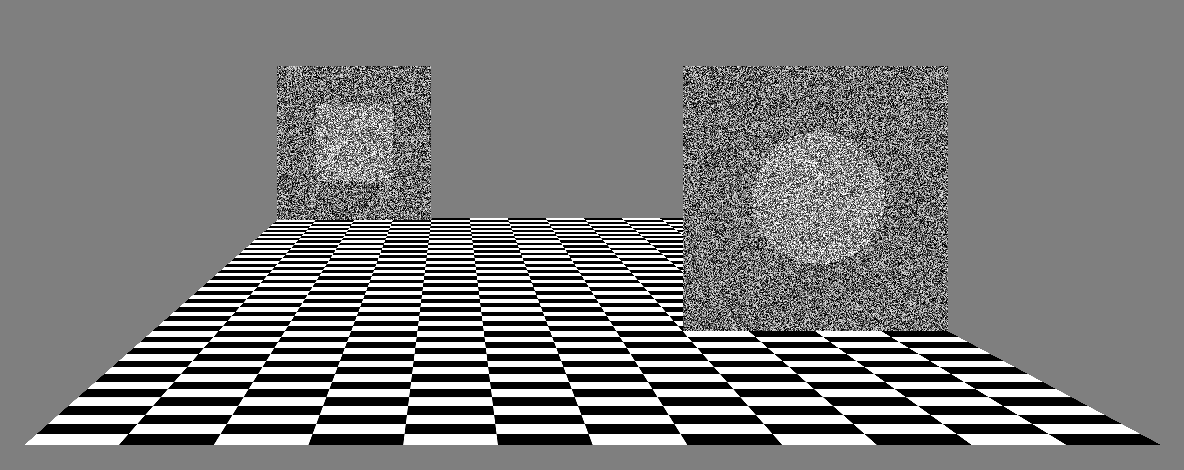
\includegraphics[width=7.5cm]{media/pilotFatigue.png}
\end{center}

\paragraph{Visual}
The test stimulus consists of a grey background (50\% grey), a continuous depth element (plane, checkerboard pattern, averaging in 50\% grey) and two random dot targets (approximately 50\% grey).
The targets show a shape which is either convex (coming out of the screen), or concave (going into the screen).
For the encoding details see section \ref{RDS}. The random pattern consists of eight shades of grey, of which the dark seven are used for the background, and the light seven for the foreground.

The random dot targets are resting on the plane, and border to either the left or the right border.
Each target can be at  one of three depth locations, at a separation of \unit[-3.1]{°}, \unit[0]{°} (parallax plane) and \unit[3.1]{°}.

The image is back-projected on a screen by two projectors through circular polarisation filters. The image height is \unit[0.7]{m}, it's width is \unit[1.17]{m}. The participant's head is at \unit[1]{m} distance of the screen, and observes the screen with polarised filter goggles. The room is dark.

\paragraph{Mechanics}
To asses the the effect of the continuous depth element, response time is logged. The other variables are the depth location of the object, the change in depth measured in angular separation, the block number and the presence of the continuous depth element.

The expected input is randomized, so concave and convex targets should be similarly common. The three depths and the two sides lead to 18 depth changes.

A cycle is built so that every depth change appears exactly once. This is achieved by pre-computing three cycles and their inverses that visit each of the six positions three times, once from each of the three nodes on the other side. Such a cycle has 18 steps, and 19 targets.
Cycles are picked at random out of the pre-computed cycles, randomly permuting the depth positions of right and left.
This gives 36 different permutations per cycle, and 216 different permutations overall.

Ten cycles form a block, either with or without continuous depth plane. The start state is chosen by the tester to counterbalance it, the presence of the depth element in later blocks is alternated.
The whole test contains 12 blocks, 2280 targets.

Before the start, after the end, and after the first six blocks, a questionnaire is presented. It consists of seven questions, with replies on a scale with six steps.


\end{multicols}

\clearpage

\begin{multicols}{2}

\tableofcontents

\end{multicols}

\appendix

\begin{thebibliography}{12}
\bibitem{AntRDS}
Bergua A., Skrandiesb W., 2000,
\textit{An early antecedent to modern random dot stereograms - 'The Secret Stereoscopic Writing' of Ram\'on y Cajal}.
Int. J. of Psychophysiology 36, 69-72\\
\url{http://dx.doi.org/10.1016/S0167-8760(99)00111-7}

\bibitem{BellRDS}
Julesz B., 1960.
\textit{Binocular depth perception of computer-generated patterns}.
Bell Syst. Tech. J. 39, 1125-1162.\\
\url{http://doi.apa.org/?uid=1961-01385-001}

\bibitem{GenRDS}
Gonzalez F., Krause F., 1994.
\textit{Generation of dynamic random-element stereograms in real time with a system based on a personal computer}.
Med. \& Biol. Eng. \& Comput., 1994, 32, 373-376.\\
\url{http://dx.doi.org/10.1007/BF02524687}

\bibitem{DepthCues}
Cutting J., Vishton P., 1995.
\textit{Perceiving layout and knowing distances: The integration, relative potency, and contextual use of different information about depth}.
In W. Epstein \& S. Rogers (Eds.), Handbook of perception and cognition, Vol. 5, 69-117. San Diego, CA: Academic Press.\\
\url{http://dx.doi.org/10.1016/B978-012240530-3/50005-5}

\end{thebibliography}

% Might only work in KOMA script (scrarticle)
\renewcommand*\refname{Links}

\begin{thebibliography}{12}
\bibitem[a]{proj} \url{http://en.wikipedia.org/wiki/Graphical_projection}
\bibitem[b]{parallel} \url{http://en.wikipedia.org/wiki/Parallel_projection}
\bibitem[c]{perspective} \url{http://en.wikipedia.org/wiki/Perspective_projection}
\bibitem[d]{painters} \url{http://en.wikipedia.org/wiki/Painter's_algorithm}
\bibitem[e]{zbuffer} \url{http://en.wikipedia.org/wiki/Z-buffering}
\bibitem[f]{fog} \url{http://www.opengl.org/documentation/specs/version1.1/glspec1.1/node90.html}
\bibitem[g]{accommodation} \url{http://en.wikipedia.org/wiki/Accommodation_(eye)}
\bibitem[h]{triangulation} \url{http://en.wikipedia.org/wiki/Triangulation}
\bibitem[i]{scenegraph} \url{http://www.realityprime.com/articles/scenegraphs-past-present-and-future}
\bibitem[j]{turing} \url{http://en.wikipedia.org/wiki/Turing_completeness}
\bibitem[k]{procedural} \url{http://en.wikipedia.org/wiki/Procedural_programming}
\end{thebibliography}




\end{document}
\end
